\chapter{Approach}
\label{approach}
I propose a two-tier approach to our problem. In the first tier, it plays the role of a \textit{filter}, and attempts to filter out the General citations, leaving behind the Specific citations to be passed to the second tier. Figure \ref{fig:twotier} illustrates the flow of our approach.
\begin{figure}[h]
  \centering
  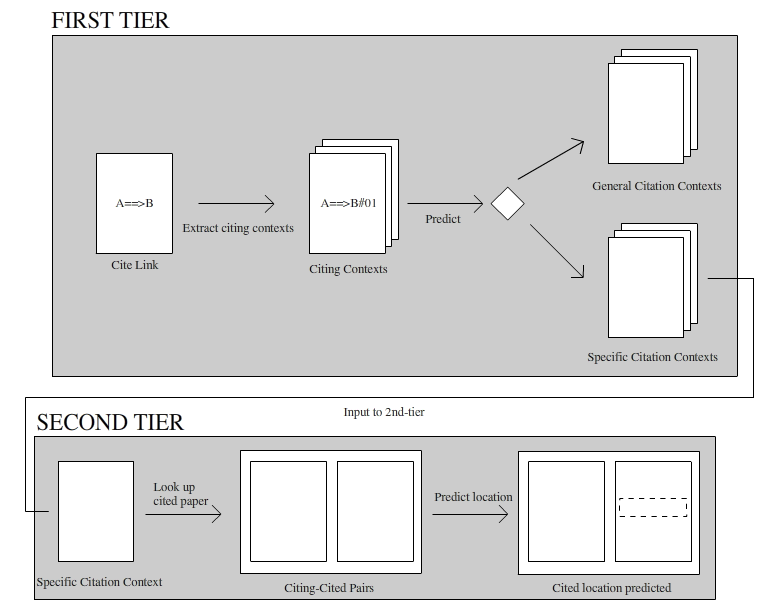
\includegraphics[scale=0.60]{./twotier}
  \caption{A Two-Tier Approach}
  \label{fig:twotier}
\end{figure}

\section{{\it GvS} (First Tier)}
\label{firsttier}
{\it GvS}, short for General versus Specific, is the first tier in my approach to filter out the General citations. In {\it GvS}, we are performing a 2-class \textit{citation classification} task, which already is a challenging task in the research area of citation analysis. We are not interested in determining whether the citation is one of the 12 class as defined by \cite{teufel2009annotation}, but only whether it is General or Specific. {\it GvS} makes use of information only from the citing contexts in a citing paper. I built a model based on features extracted from the citing contexts. With this model, {\it GvS} classifies citing contexts into one of the two classes. Only those contexts that are classified as Specific will be passed to the second tier.

\subsection*{Building The Model For {\it GvS}}
To build a model to classify General versus Specific, we adopt some of the features that \cite{dongensemble} used for citation classification. From each of the 275 annotated cite links mentioned in Table \ref{tab:annotation} I extract a set of features into a {\it feature vector} and map it to its {\it label} according to annotation (Figure \ref{fig:featurevector}). The features used are as described below.

\begin{figure}[h]
\centering
$v_1:[f_1, f_2, f_3, \ldots, f_n] \rightarrow L_1$ \\
$v_2:[f_1, f_2, f_3, \ldots, f_n] \rightarrow L_2$ \\
$\vdots$ \\
$v_i:[f_1, f_2, f_3, \ldots, f_n] \rightarrow L_i$ \\
$\vdots$ \\
$v_m:[f_1, f_2, f_3, \ldots, f_n] \rightarrow L_m$
\caption{Mapping feature vectors to labels from annotation}
\label{fig:featurevector}
\end{figure}

\subsection*{{\it GvS} Features}
\begin{enumerate}
\item Physical Features \\
We adopted the physical features as presented in \cite{dongensemble}. They are:
\begin{enumerate}
\item \textit{Location}: in which section the citing sentence is from.
\item \textit{Popularity}: no. of citation marks in the citing sentence.
\item \textit{Density}: no. of unique citation marks in the citing sentence and its neighbour sentences.
\item \textit{AvgDens}: the average of Density among the citing and neighbour sentences.
\end{enumerate}
The intuition I have for using this feature is: A higher number of citation marks within a citing sentence suggests these citations are likely to be General since there was little room of discussion by the author(s).

\item Number Density \\
A numerical feature similar to the first feature set that measures the density of numerical figures in the citing context. The intuition is that Specific citations tend refer numerical figures in evaluation results in the cited paper. E.g. ``...Nivre and Scholz (2004) obtained a precision of 79.1\%...". This feature was added based on the observations I made earlier in Chapter \ref{buildingcorpus}.

\item Publishing Year Difference \\
A numerical feature that represents difference in the publishing year between the citing and cited paper. The intuition is that higher difference suggests cited paper is older and presented a fundamental idea, and thus cited for General purposes.

\item Citing Context's Average \url{tf-idf} Weight \\
A numerical feature that indicates the average amount of \textit{valuable} words, as determined by \url{tf-idf} \cite{irtextbook},  in the citing context. Higher values suggest important words and thus specific keywords.

\item Cue Words \\
Another numerical feature adopted from \cite{dongensemble}, that computes the amount of cue words that appear in the citing sentence and its neighbour sentences. We defined 2 classes of cue words: Cue-General and Cue-Specific (refer to Appendix \ref{cuewords} for list of cue words). These cue words are hand-picked based on the examples I observed during the annotation process.
\end{enumerate}

Recall that according to our annotation statistics, this task is heavily skewed towards General citations. Building a model based on this skewed set of data instances will only produce a bias model that often predicts General. In fact, during some preliminary experiments where all data instances are fitted into the model, it outputs General for all its predictions. To fix this problem, I propose training the model on unskewed data.

From the set of labelled feature vectors, I first gathered the Specific instances. Then I {\bf randomly} selected from the rest to have a $1:1$ of Specific vs General instances. While this ratio appear unrealistic compared to the actual statistics, I argue that I am building a model using balanced data to measure its ability to differentiate between the 2 types of citation.

\section{{\it LocateProv} (Second Tier)}
{\it LocateProv}, short for Locate Provenance, is the second tier of my approach. The design of {\it LocateProv} is all its inputs are Specific citations predicts which of the fragments in the cited paper is the cited fragment. Resembling a search, in {\it LocateProv} the citing context becomes the {\it query} to match the cited fragments in the cited paper. For that I also added some features that are common in Information Retrieval tasks.

\subsection*{Building The Model For {\it LocateProv}}
In {\it LocateProv} we are predicting which cited fragment is the provenance of a citation. Instead of cite links, I used the annotated fragments in Table \ref{tab:annotation} to build the model. In this tier the features used are based on both the citing contexts and the cited fragments in order to {\it connect} the citation to its provenance. Similarly the feature vectors are mapped onto the annotated labels.

\subsection*{{\it LocateProv} Features}
\begin{enumerate}
\item Surface Matching \\
A numerical feature that measures the amount of word overlap between the citing sentence and a fragment in the cited paper.

\item Number Near-Miss \\
A numerical feature that measures the amount of numerical figures overlap between the citing sentence and a fragment in the cited paper. This feature will preprocess each fragment, rounding numerical figures or converting to percentage values when it tries to match the numerical figures in the citing sentence. This feature was added because of the observations I made earlier in Chapter \ref{buildingcorpus}, that citations may refer to evaluation results in the cited paper.

\item Bigrams Matching \\
A numerical feature that measures the amount of bigrams overlap between the citing sentence and a fragment in the cited paper. This feature was added to preserve word order when comparing the citing sentence and the fragment. This feature was also targeted at Specific citations that refer to term definitions or quote directly.

\item Cosine Similarity \\
A common numerical feature used in Information Retrieval tasks to measure similarity between the query and a candidate document. In our case, citing sentence and the fragment.
\end{enumerate}
Most of these features are added based on some of the observations I made during the annotation tasks.

Again, recall that the data instances that were annotated are heavily skewed against Specific citations. In fact, the ratio of Specific-Yes instances compared to the rest is at least $1:1000$. It is impossible to train a model that is not bias with this entire set of instances. Hence I used the same method used in {\it GvS}: to use a $1:1$ of Specific-Yes versus Specific-No instances. Note that this also coincide with the design of {\it LocateProv} that inputs are only Specific citations. It was also not feasible to use the actual ratio between Specific-Yes and Specific-No because comparing a citing-cited pair of papers, the ratio of citing context to the number of fragments in the cited paper is easily $1:100$.

For both tiers, I trained the models using various classifiers and evaluated their performances on a few evaluation strategies. I discuss the evaluation scheme in the following chapter.